\documentclass[12pt]{book}
\usepackage[utf8]{inputenc}
\usepackage[margin=1.25in]{geometry}
\usepackage{graphicx}
\usepackage{amsmath , amssymb ,ragged2e}
\usepackage{bm}
\usepackage{esvect}
\usepackage{centernot}
\usepackage[usestackEOL]{stackengine}
\usepackage{eqparbox} 

\begin{document}
    \chapter{Introduction}
        \subsection{Introduction}
            \begin{itemize}
                \item Astrologie $ \implies $ art, pas une science
                \item Astronomie $ \implies $ science d'observation et de mesures 
                \item Cosmologie $ \implies $ etude de la structure et de l'evolution de l'univers
                \item Astrophysique $ \implies $ les lois de physique vs observation
            \end{itemize}
        \subsection{Les unites de distance}
            \begin{itemize}
                \item unite astronomique (U.A.) : $ 1.\text{U.A}=1,5\times 10^{11}m $ ( pour des distances dans le systeme solaire) \\
                    1U.A = distance moyenne entre Terre soleil
                \item annee lumineuse (a.l.) : $ 1.\text{a.l.} = 63240 \text{U.A.} = 9,46\times 10 ^{15} $ ( distances entre etoiles dans la meme galaxie)
                \item parsec (pc) : $ 1.\text{pc} = 3,26.\text{a.l.}=3,1\time 10^{16} m$ ( distances entre galaxies)
            \end{itemize}
        \pagebreak
        \subsection{Systeme solaire et planetes}
            \begin{itemize}
                \item soleil
                \item mercure
                \item venus
                \item Terre
                \item mars
                \item jupiter
                \item saturne 
                \item uranus
                \item neptune
                \item pluto
            \end{itemize}
            La zone habituble dans le systeme solaire et entre Venus et Mars \\ 
            Tous qui est plus loin que Neptune est considere (trans neptunian objects)\\
            Notre (systeme solaire) il est a 8 Kpc du centre de la galaxie
    \chapter{Sphere celest}
        \begin{minipage}{0.65\linewidth}
            Geocentriquement , La terre se trouve dans une spher celeste , les etoiles semblent etre fixes sur cette sphere qui tourne autour de la terre \\ 
            La terre tourne de ouest ver l'est , la sphere celest apparait en rotation d'est vers l'ouest autour de l'axe de la terre \\
            l'axe de la terre est pinte vers polaris , avec une difference de 0,75 degree
        \end{minipage}
        \begin{minipage}{0.34\linewidth}
            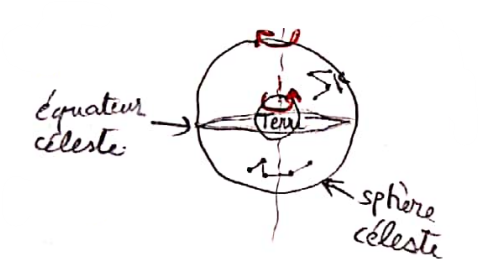
\includegraphics[width=\linewidth]{pic/spherecelest.png}
        \end{minipage}
        Pour determiner les coordonnees d'une etoile sur la sphere celeste , on a 2 type de coordonnees 
            \begin{itemize}
                \item coordone locales (altitude , azimuth)\\ 
                    \begin{center}
                        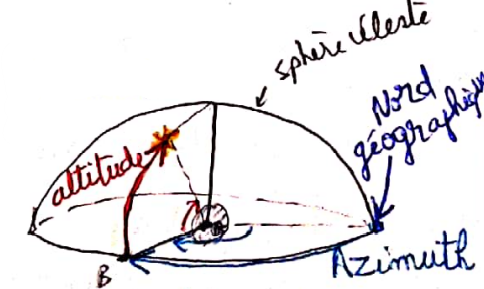
\includegraphics[width=0.3\linewidth]{pic/spherecelestcoordone1.png}
                    \end{center}
                    
                \item coordone equatorials (dclinaison , ascension droite)\\ 
                    \begin{center}
                        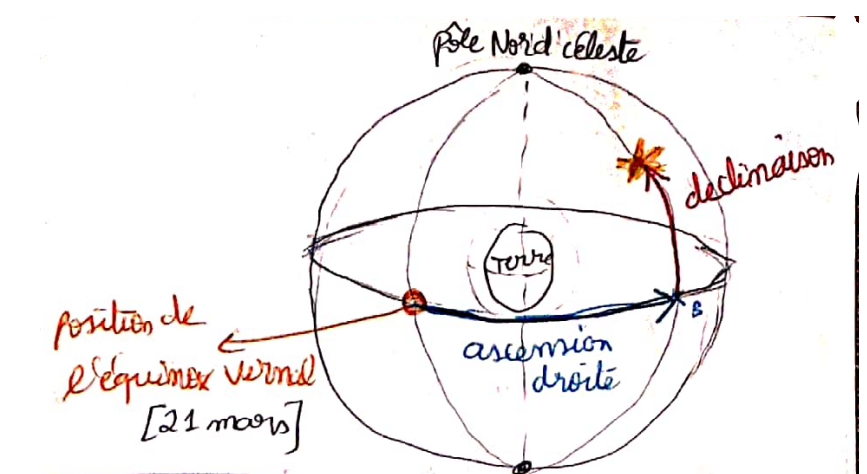
\includegraphics[width=0.3\linewidth]{pic/spherecelestcoordone2.png}
                    \end{center}
                    
            \end{itemize}
            \pagebreak
        \begin{itemize}
            \item \underline{Constellation} : groupe d'etoiles voisines , presentant une figure conventionnelle determinee , a laquelle on a donne un nom particulier 
            \item\underline{Amas (clusters)} : groupe d'etoiles liees par gravite 
            \item\underline{asterisme} : sous-groupe d'etoiles d'une constellation 
            \item\underline{etoilles (constellations) circompolaires}: ne descendent jamais sou l'horizon et peuvent etre vus toute l'annee 
            \item\underline{U.I.A.} : International Astonomical Union, designe 88 constellations dans tout le ciel
            \item\underline{eliptique} : le trajet de rotation de laterre autour du soleil \\ 
            \underline{Note :} la terre est incline par 23.5 degree $ \implies $ l'eciptique est incline par 23,5 degree par raport a l'equateur celeste 
            \item\underline{Zodiac } : ce sont 12 constellation de les 88 , les plus proches des d'ecliptique , qui sont a de largeur (18 degree ( 8 (desous de l'ecliptique)+ 8 (dessus de l'ecliptique) + 2 ( pour l'erreur)))
            \item\underline{Nominisatoin des l'etoiles selon la brillance} : $ \alpha \implies $ la plus brillante , $ \beta \implies  $ la seconde brillante ...
        \end{itemize}
    \chapter{Les saisons}
        Mouvement de la terre \begin{itemize}
            \item Rotation (autour de son axe)
            \item Revolution ( autour du soleil)
        \end{itemize}
        annee terrestre : temps mis par la terre pour effectuer 1 tour autour du soleil (365,25 jours)
        \begin{itemize}
            \item Jour sideral : 23h 56 min : temps mis par la terre pour effectuer 1 cycle complet autour de son axe 
            \item Jour solaire : 24 h : temps aubout duquel la terre retrouve sa position precedente par rapport a la soleil \\
                $ J_{\text{solaire}} = J_{\text{sideral}} + 4 $
        \end{itemize}
        La duree du jour solaire sur une planete : $ \frac{1}{J_{\text{solair}}} = \frac{1}{J_{\text{sideral}}} - \frac{1}{A_{\text{sideral}}} $ \\
        Si $ J_\text{solair} > 0 \implies  $ rotation de planete est anticlock wise\\
        Si $ J_\text{solair} < 0 \implies  $ rotation de planete est clock wise \\
        \pagebreak
        L 'inclinaison de l'axe de la terre de 23,5 degree cause les saison\\
            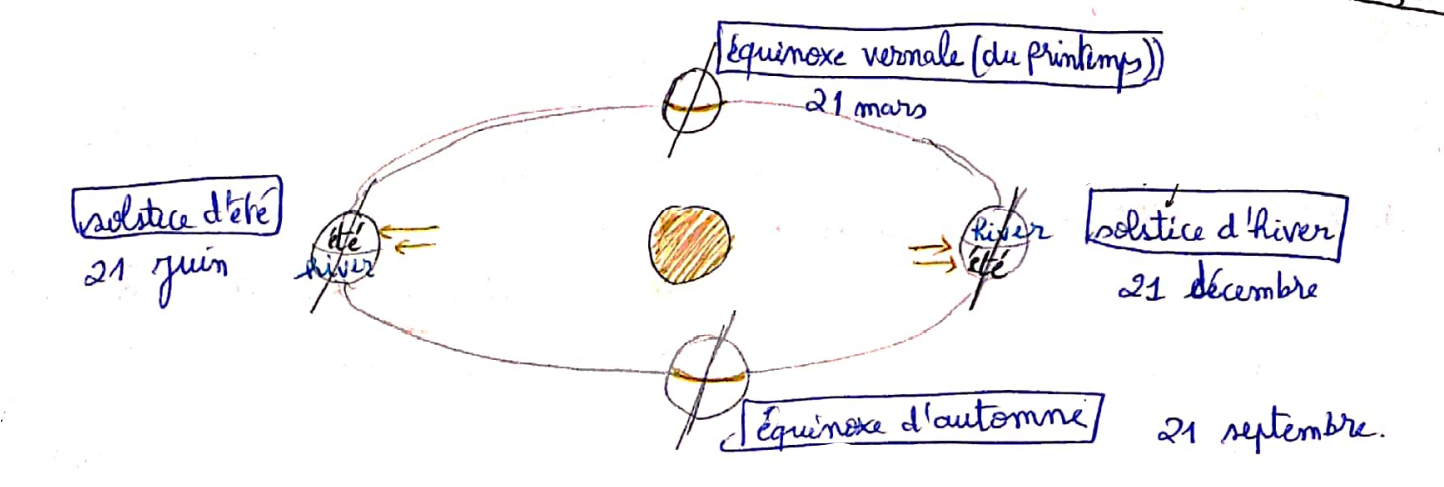
\includegraphics[width=1\linewidth]{pic/seasons.png}
            \begin{itemize}
                \item Pendant l'equinoxe le jour = le nuit 
                \item Pendant le solstice d'hiver le jour < le nuit 
                \item Pendant le solstice d'ete le jour > le nuit 
            \end{itemize}
        \begin{minipage}{0.65\linewidth}
            Il existe entre la terre et la lune une forces d'attraction , maintenant , laxe de la terre pinte vers polaris ,dans 13 00 ans , il pointera vers Vega
        \end{minipage}
        \begin{minipage}{0.34\linewidth}
            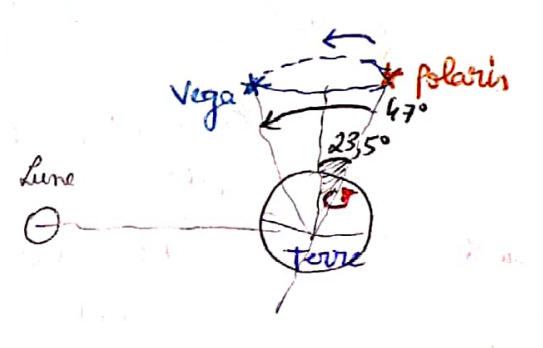
\includegraphics[width=\linewidth]{pic/vega.png}
        \end{minipage}
    \chapter{Les eclipses}
        \begin{itemize}
            \item Eclipse lunair\\
                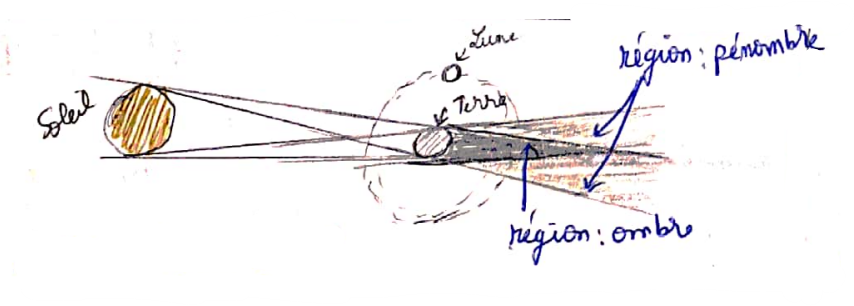
\includegraphics[width=0.7\linewidth]{pic/lunaireclipse.png}
                \begin{itemize}
                    \item penombrale : la lune est dans le penombre 
                    \item partielle : partie de la lune est dans l'ombre, l'aure partie dans le penombre 
                    \item total : la lune entiere est dans l'ombre
                \end{itemize}
                Condition de l'eclipse lunaire : \begin{itemize}
                    \item lune dans la phase "plaine lune"
                    \item Soleil , Terre et Lune alignes sur la ligne node
                \end{itemize}
            \item Eclipse solaire\\
                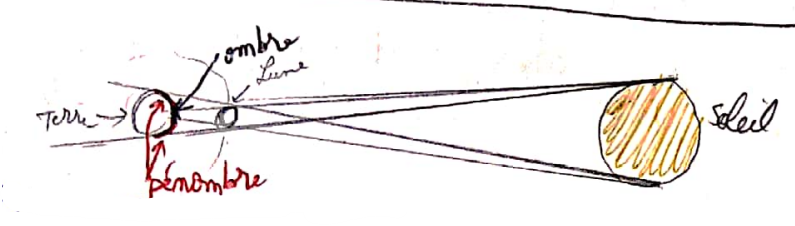
\includegraphics[width=0.7\linewidth]{pic/solaireclipse.png}
                \begin{itemize}
                    \item totale : Le sommet du cone d'ombre est sur ou au dessous de la terre 
                        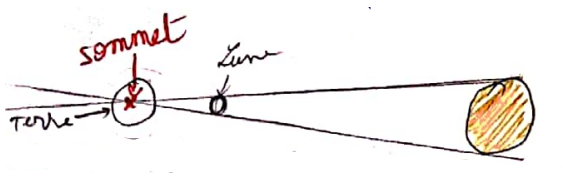
\includegraphics[width=0.3\linewidth]{pic/solareclipstotal.png}
                    \item annulaire :le sommet du cone d'ombre est au dessus de la terre \\
                        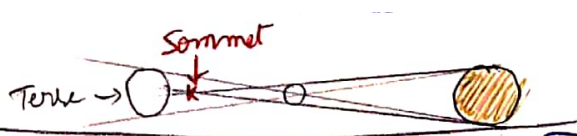
\includegraphics[width=0.3\linewidth]{pic/solareclipsannulair.png}
                \end{itemize}
                Condition de l'eclipse solaire \begin{itemize}
                    \item lune dans la phase " Nouvelle lune "
                    \item Lune Soleil , Terre alignes
                \end{itemize}
        \end{itemize}
        Chaque 5,4 mois il y aura une eclipse (lunaire ou solaire ) a un endroit de la terre 
        \section{periodicite des eclipses : cycle saros}
            Chaque eclipse appartient a une serie de Saros . Chaque Saros est lie a une disposition de la ligne de noeuds \\
            Cycle de Saros : \\
                \begin{itemize}
                    \item la meme eclipse se pase a une periode de 18 ans + (11-$ \frac{1}{3} $)jours = 223 mois lunairs 
                    \item ces eclipse ne se produisent pas exactement au meme endroit au cours des cycle de saros 
                    \item apres 3 saros , une eclipse se produit sur la meme partie de la terre
                \end{itemize}
        
        




\end{document}